% Options for packages loaded elsewhere
\PassOptionsToPackage{unicode}{hyperref}
\PassOptionsToPackage{hyphens}{url}
%
\documentclass[
  11pt,
]{article}
\usepackage{amsmath,amssymb}
\usepackage{iftex}
\ifPDFTeX
  \usepackage[T1]{fontenc}
  \usepackage[utf8]{inputenc}
  \usepackage{textcomp} % provide euro and other symbols
\else % if luatex or xetex
  \usepackage{unicode-math} % this also loads fontspec
  \defaultfontfeatures{Scale=MatchLowercase}
  \defaultfontfeatures[\rmfamily]{Ligatures=TeX,Scale=1}
\fi
\usepackage{lmodern}
\ifPDFTeX\else
  % xetex/luatex font selection
    \setmainfont[]{Times New Roman}
\fi
% Use upquote if available, for straight quotes in verbatim environments
\IfFileExists{upquote.sty}{\usepackage{upquote}}{}
\IfFileExists{microtype.sty}{% use microtype if available
  \usepackage[]{microtype}
  \UseMicrotypeSet[protrusion]{basicmath} % disable protrusion for tt fonts
}{}
\makeatletter
\@ifundefined{KOMAClassName}{% if non-KOMA class
  \IfFileExists{parskip.sty}{%
    \usepackage{parskip}
  }{% else
    \setlength{\parindent}{0pt}
    \setlength{\parskip}{6pt plus 2pt minus 1pt}}
}{% if KOMA class
  \KOMAoptions{parskip=half}}
\makeatother
\usepackage{xcolor}
\usepackage[margin=1in]{geometry}
\usepackage{longtable,booktabs,array}
\usepackage{calc} % for calculating minipage widths
% Correct order of tables after \paragraph or \subparagraph
\usepackage{etoolbox}
\makeatletter
\patchcmd\longtable{\par}{\if@noskipsec\mbox{}\fi\par}{}{}
\makeatother
% Allow footnotes in longtable head/foot
\IfFileExists{footnotehyper.sty}{\usepackage{footnotehyper}}{\usepackage{footnote}}
\makesavenoteenv{longtable}
\usepackage{graphicx}
\makeatletter
\def\maxwidth{\ifdim\Gin@nat@width>\linewidth\linewidth\else\Gin@nat@width\fi}
\def\maxheight{\ifdim\Gin@nat@height>\textheight\textheight\else\Gin@nat@height\fi}
\makeatother
% Scale images if necessary, so that they will not overflow the page
% margins by default, and it is still possible to overwrite the defaults
% using explicit options in \includegraphics[width, height, ...]{}
\setkeys{Gin}{width=\maxwidth,height=\maxheight,keepaspectratio}
% Set default figure placement to htbp
\makeatletter
\def\fps@figure{htbp}
\makeatother
\setlength{\emergencystretch}{3em} % prevent overfull lines
\providecommand{\tightlist}{%
  \setlength{\itemsep}{0pt}\setlength{\parskip}{0pt}}
\setcounter{secnumdepth}{-\maxdimen} % remove section numbering
% definitions for citeproc citations
\NewDocumentCommand\citeproctext{}{}
\NewDocumentCommand\citeproc{mm}{%
  \begingroup\def\citeproctext{#2}\cite{#1}\endgroup}
\makeatletter
 % allow citations to break across lines
 \let\@cite@ofmt\@firstofone
 % avoid brackets around text for \cite:
 \def\@biblabel#1{}
 \def\@cite#1#2{{#1\if@tempswa , #2\fi}}
\makeatother
\newlength{\cslhangindent}
\setlength{\cslhangindent}{1.5em}
\newlength{\csllabelwidth}
\setlength{\csllabelwidth}{3em}
\newenvironment{CSLReferences}[2] % #1 hanging-indent, #2 entry-spacing
 {\begin{list}{}{%
  \setlength{\itemindent}{0pt}
  \setlength{\leftmargin}{0pt}
  \setlength{\parsep}{0pt}
  % turn on hanging indent if param 1 is 1
  \ifodd #1
   \setlength{\leftmargin}{\cslhangindent}
   \setlength{\itemindent}{-1\cslhangindent}
  \fi
  % set entry spacing
  \setlength{\itemsep}{#2\baselineskip}}}
 {\end{list}}
\usepackage{calc}
\newcommand{\CSLBlock}[1]{\hfill\break\parbox[t]{\linewidth}{\strut\ignorespaces#1\strut}}
\newcommand{\CSLLeftMargin}[1]{\parbox[t]{\csllabelwidth}{\strut#1\strut}}
\newcommand{\CSLRightInline}[1]{\parbox[t]{\linewidth - \csllabelwidth}{\strut#1\strut}}
\newcommand{\CSLIndent}[1]{\hspace{\cslhangindent}#1}
\ifLuaTeX
  \usepackage{selnolig}  % disable illegal ligatures
\fi
\usepackage{bookmark}
\IfFileExists{xurl.sty}{\usepackage{xurl}}{} % add URL line breaks if available
\urlstyle{same}
\hypersetup{
  pdftitle={The Stability/Flexibility Tradeoff On Task-switching},
  pdfauthor={Sophia Angleton, Fiona Debernardi, Stephen Anti},
  hidelinks,
  pdfcreator={LaTeX via pandoc}}

\title{The Stability/Flexibility Tradeoff On Task-switching}
\author{Sophia Angleton, Fiona Debernardi, Stephen Anti}
\date{2024-12-11}

\begin{document}
\maketitle

{
\setcounter{tocdepth}{2}
\tableofcontents
}
\subsection{Abstract}\label{abstract}

This study is interested in understanding the relationship between
task-switching and the cognitive stability-flexibility tradeoff. The
design of this study will involve task-switching in an alternating runs
manner, where there are two cues this task switches between, shape and
color and these alternate in cycles of 4, each run being cycles of 4.
This study will use alternating runs task-switching to understand the
relationship between cognitive stability and cognitive flexibility. We
will use the stability-flexibility tradeoff to inform our predictions,
where we predict that 1) There is a negative relationship between
expression of stability and expression of flexibility. We will see this
relationship on three levels, within-subjects, in individual
differences, and on the experimental level. Through a basic analysis of
data, we saw there was a difference between stability and flexibility
through a difference in switch cost measured in response time. This
shows that there is a presence of stability and flexibility informing
our task-switching study, however further analysis is required to
understand the directionality of the relationship.

\subsection{Introduction}\label{introduction}

The paradigm between cognitive stability and cognitive flexibility is a
widely known and established relationship in the world of cognitive
science. Both cognitive stability and flexibility are aspects of
executive functioning, or what we understand as self-control (Monsell
and Driver 2000). Cognitive flexibility centers itself in a domain of
executive functioning called mental set shifting, and in previous
literature, has been understood through the use of the task-switching
paradigm. Tasks such as odds-evens, the Stroop task, or other
alternating tasks where through the use of cues, participants need to
identify an alternating attribute of a stimuli (Mayr, Kuhns, and Hubbard
2014). For this study, the task-switch paradigm is constructed through
the identification of one of two attributes, color or shape, where they
identify color of the stimulus or shape of the stimulus, respectively.
According to the established stability/flexibility tradeoff, when one is
performing a task that requires more cognitive stability, it is harder
to also be more cognitively flexible. This is seen in the task-switch
paradigm within-subjects where they have less switch-costs when not
switching task cues compared to higher switch-costs when switching from
one cue to another (Mayr and Grätz 2024).

However, a recent reevaluation of the generalizability of the
stability/flexibility tradeoff has posited that tradeoffs originally
thought to explain a plethora of cognitive models, occur only in highly
specified contexts (Mayr and Grätz 2024). Instead, there is newfound
evidence of an anti-tradeoff pattern, meaning there is co-occurrence of
cognitive stability and flexibility depending on the level of resolution
encoding (Mayr and Grätz 2024). These recent findings in the field of
decision-making suggest that the stability-flexibility trade off may not
be as strong as once thought, however in this study we are still
predicting we will see a negative relationship between the switch
(flexibility) and no-switch (stability) variables through a comparison
of error rate and response time until further studies explain more about
a potential anti-tradeoff occurring. Indeed, using the
stability-flexibility tradeoff to inform our predictions, we predict
that: 1) There is a negative relationship between expression of
stability and expression of flexibility. We will see this relationship
on three levels, within-subjects, in individual differences, and on the
experimental level. We will calculate the difference in reaction times
between no-switch and switch trials. A smaller reaction time difference
is interpreted as a higher level of stability, whereas a longer reaction
time indicates a higher level of flexibility (Monsell and Driver 2000).

\subsection{Methods}\label{methods}

\subsubsection{Data Cleaning}\label{data-cleaning}

Using RStudio, the first major step for analyzing the dataset involved a
clean-up process. The first clean up involved re-naming columns for
better understanding of the dataset. Variables dim1 was replaced with
dimshape, dim2 replaced with dimcolor, time replaced with RT, cor with
correct, and res with response. Following from that, numeric values in
the dataset were replaced with character strings for the variables Task
and Error. Practice trials were then removed from the dataset since the
ultimate for the final data is to isolate switch trials and control
trials.

\subsubsection{Determine and Remove
Outliers}\label{determine-and-remove-outliers}

\paragraph{Outliers by Error:}\label{outliers-by-error}

Since a key task of this study is to test for accuracy, it was necessary
to operationalize accuracy by setting a criterion of 80\% accuracy in
all trials per participant. Out of the total of 896 trials, and using
the 80\% accuracy limit, at least 179 were needed to meet the accuracy
threshold denoted by 0 in the error variable column. Grouping by id and
summing by error and filtering out all those falling below the accuracy
threshold, two people fellow below the accuracy threshold and were
removed (id : 70 and id: 87). These two were the outliers by error.

\subsubsection{Outliers by
Inter-response}\label{outliers-by-inter-response}

A close inspection of the data and examining RT variable in descending
order, showed that some participants only did 7 blocks of runs instead
of 8. To account for this variance, the z-score for each sequence
position along with switch and ambiguity were run on the RT variable and
Z-Score was also run on each block.

To arrive at this, the first step was to separate switch trials, c(1,5)
and control trials !c(1,5). This means, if task is 1 or 5, we assigned
switch, else, it was assigned as control. First trial after each block
had to be thrown out because it is not a switch or no-switch. Cycle
positions were separated into cycle positions of 4, making a total of 16
conditions.

\subsection{Mean and Standard Error of Response
Time}\label{mean-and-standard-error-of-response-time}

Second step involved calculating mean response times (RT) by trial type
and calculating the z-scores. The z-score for both control and switch
was 0 (the expected value) and that our Z-Standard Deviation (Zsd) is 1
(which is also the expected value ). Looking at the mean for RT in both
switch and control shows that the response time means tend to be a lot
longer on average than the average response time for control trials
(non-switch trials). The difference in means was by 311 where the switch
trial takes 311 ms longer than the control or non-switch trials.

Outliers were identified for z-scores (scores beyond -3 and 3), means
and standard error of response time for each trail type was also
calculated.

\subsection{Results}\label{results}

First, we created a density plot to examine how response times (RT) were
distributed in the data set (See Figure 1). We wanted to first examine
how participants were responding across all conditions, so we averaged
participants response times and then put them into this density plot.
The average response time (as indicated by the red dashed line) was 860
ms and the standard deviation was 697 ms.

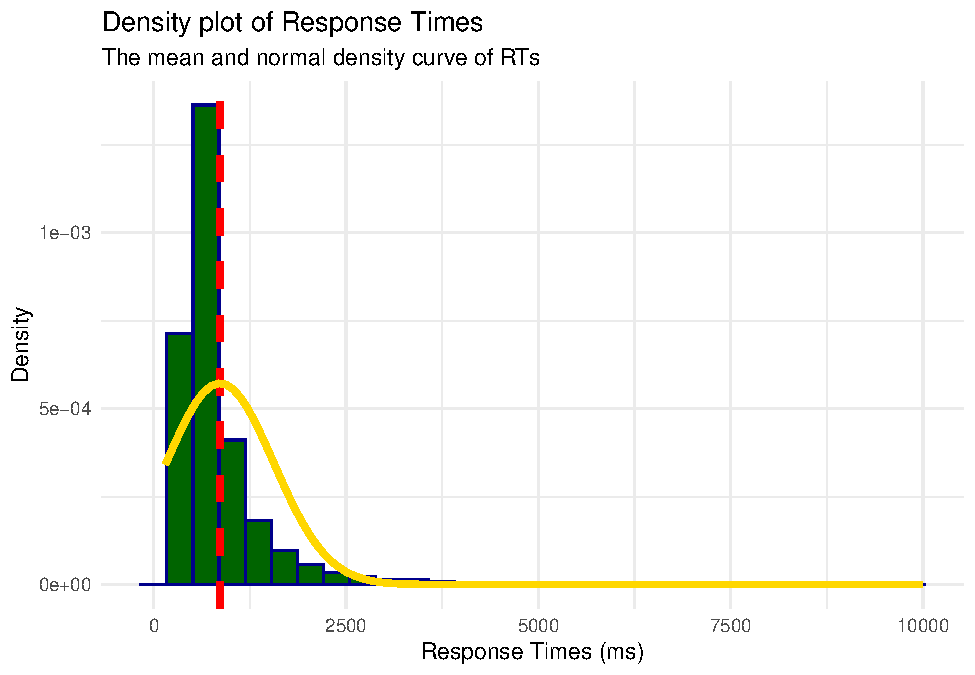
\includegraphics{final_paper_EDLD_files/figure-latex/unnamed-chunk-3-1.pdf}

Next, we examined whether the participants' response times in the
control condition varied from their response times in the switch
condition. We found that average response time varied by condition. In
the control condition, participants responded more quickly (M = 748, SD
= 581). In the switch condition, participants had slower response times
(M = 1186, SD = 891). We pivoted the data to create separate columns for
each condition, and then we calculated the mean and standard deviation
of each column. We then created a table to depict these descriptives.

\begin{longtable}[]{@{}lrr@{}}
\caption{Descriptive Statistics for Response Times}\tabularnewline
\toprule\noalign{}
Statistic & Response\_time\_control & Response\_time\_switch \\
\midrule\noalign{}
\endfirsthead
\toprule\noalign{}
Statistic & Response\_time\_control & Response\_time\_switch \\
\midrule\noalign{}
\endhead
\bottomrule\noalign{}
\endlastfoot
Mean & 747.59 & 1186.02 \\
Median & 596.00 & 916.00 \\
Standard Deviation & 580.69 & 891.09 \\
\end{longtable}

Finally, we created a bar chart to show the difference in response times
by condition. This chart is another way of visualizing the results that
we found above. The chart shows that when participants were told by the
instructions to switch from one task to another (switch trial), they
took longer than when they were doing the same task repeatedly (control
trial).

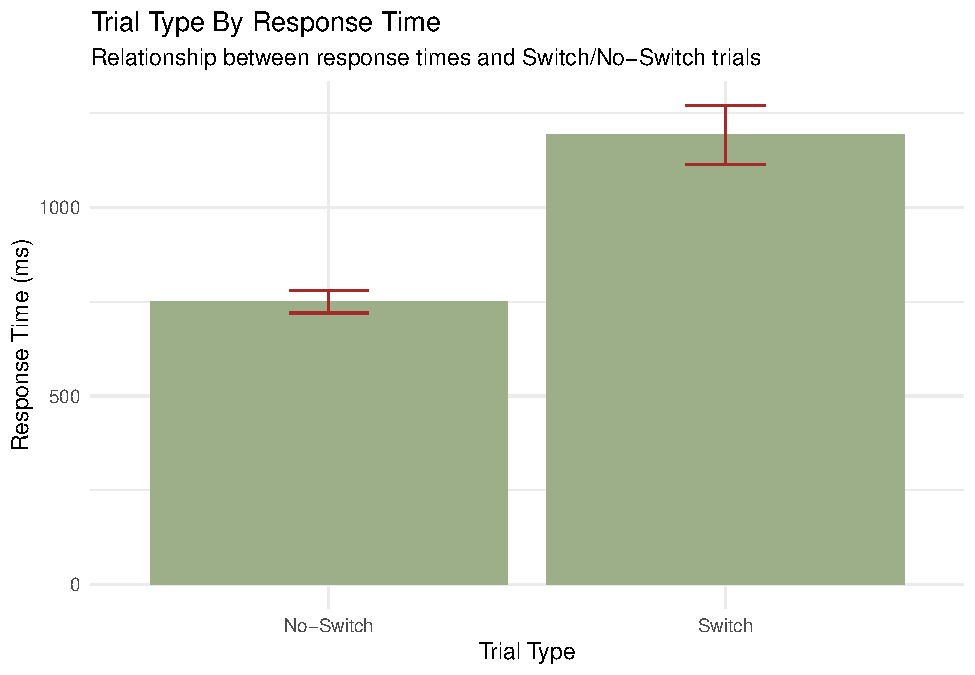
\includegraphics{final_paper_EDLD_files/figure-latex/unnamed-chunk-6-1.pdf}

\subsection{Discussion}\label{discussion}

The main goal of this study was to investigate task-switching and the
trade off between cognitive stability and flexibility. The overall
takeaway is that when participants need to switch instructions, their
reaction times to the tasks are slower compared to when they are doing
the same task repeatedly. In the future, more research is needed to
examine whether the differences in responses to the conditions are
statistically significant.

\newpage

\subsection*{References}\label{references}
\addcontentsline{toc}{subsection}{References}

\phantomsection\label{refs}
\begin{CSLReferences}{1}{0}
\bibitem[\citeproctext]{ref-mayr_does_2024}
Mayr, Ulrich, and Dominik Grätz. 2024. {``Does Cognitive Control Have a
General Stability/Flexibility Tradeoff Problem?''} \emph{Current Opinion
in Behavioral Sciences} 57 (June): 101389.
\url{https://doi.org/10.1016/j.cobeha.2024.101389}.

\bibitem[\citeproctext]{ref-mayr_long-term_2014}
Mayr, Ulrich, David Kuhns, and Jason Hubbard. 2014. {``Long-Term Memory
and the Control of Attentional Control.''} \emph{Cognitive Psychology}
72 (July): 1--26. \url{https://doi.org/10.1016/j.cogpsych.2014.02.001}.

\bibitem[\citeproctext]{ref-monsell_control_2000}
Monsell, Stephen, and Jon Driver. 2000. \emph{Control of {Cognitive}
{Processes}: {Attention} and {Performance} {XVIII}}. The MIT Press.
\url{https://doi.org/10.7551/mitpress/1481.001.0001}.

\end{CSLReferences}

\end{document}
